\section{System-wide Profiling \& Tracing}

\begin{frame}
  \frametitle{System-wide Profiling \& Tracing}
  \begin{itemize}
    \item Sometimes, the problems are not tied to an application but rather
          due to the usage of multiple layers (drivers, application, kernel).
    \item In that case, it might be useful to analyze the whole stack.
    \item The kernel already includes a large number of tracepoints that can be
          recorded using specific tools.
    \item New tracepoints can also be created statically or dynamically using
          various mechanisms (kprobes for instance).
  \end{itemize}
\end{frame}

\subsection{kprobes}

\begin{frame}[fragile]
  \frametitle{Kprobes}
  \begin{itemize}
    \item Allows to insert breaks at almost any kernel address
          dynamically and to extract debugging and performance
          information
    \item Uses code patching to modify text code to insert calls to specific
          handlers
    \begin{itemize}
      \item \code{kprobes} allows to execute specific handlers when the hooked
            instruction is executed
      \item \code{kretprobes} will trigger when returning from a function allowing to
            extract the return value of functions but also display the
            parameters that were used for the function call
    \end{itemize}
    \item Needs some basic kernel configuration:
	    \begin{itemize}
		    \item \kconfigval{CONFIG_KPROBES}{y} to enable general
			    kprobe support
		    \item \kconfigval{CONFIG_KALLSYMS_ALL}{y} to allow
			    hooking probes using \code{<symbol_name>}
			    instead of raw function address
		    \item \kconfigval{CONFIG_KPROBE_EVENTS}{y} to enable
			    kprobes usage as tracing events in
			    \code{tracefs}
	    \end{itemize}
    \item At the lowest level, k(ret)probes are manipulated with dedicated
	    kernel APIs, allowing to write our own kprobe tools (eg as
	    kernel modules)
    \item Can also be used from userspace with
	    \code{/sys/kernel/tracing/kprobe_events}
    \item See \kdochtml{trace/kprobes} for more information
  \end{itemize}
\end{frame}

\begin{frame}[fragile]{Basic kprobe tracing (1/2)}
	\begin{itemize}
		\item Add a kprobe on \code{do_sys_openat2}:
	\end{itemize}
	\begin{block}{}
		\begin{minted}[fontsize=\footnotesize]{console}
$ echo "p:my_probe do_sys_openat2" > /sys/kernel/tracing/kprobe_events
		\end{minted}
	\end{block}
	\begin{itemize}
		\item Add a kprobe in the same function but at a specific
			offset, and capture some arguments
	\end{itemize}
	\begin{block}{}
		\begin{minted}[fontsize=\footnotesize]{console}
$ echo "p:my_probe_2 do_sys_openat2+0x7c file=%r2" > /sys/kernel/tracing/kprobe_events
		\end{minted}
	\end{block}
	\begin{itemize}
		\item Insert a kretprobe
	\end{itemize}
	\begin{block}{}
		\begin{minted}[fontsize=\footnotesize]{console}
$ echo 'r:my_retprobe do_sys_openat2 $retval' > /sys/kernel/tracing/kprobe_events
		\end{minted}
	\end{block}
\end{frame}

\begin{frame}[fragile]{Basic kprobe tracing (2/2)}
	\begin{itemize}
		\item Show existing kprobes
	\end{itemize}
	\begin{block}{}
		\begin{minted}[fontsize=\footnotesize]{console}
$ cat /sys/kernel/tracing/kprobe_events
		\end{minted}
	\end{block}
	\begin{itemize}
		\item Enable a kprobe (ie: start capturing the
			corresponding event)
	\end{itemize}
	\begin{block}{}
		\begin{minted}[fontsize=\footnotesize]{console}
$ echo 1 > /sys/kernel/tracing/events/kprobes/my_probe/enable
		\end{minted}
	\end{block}
	\begin{itemize}
		\item Get data emitted by kprobes
	\end{itemize}
	\begin{block}{}
		\begin{minted}[fontsize=\footnotesize]{console}
$ cat /sys/kernel/tracing/trace
		\end{minted}
	\end{block}
	\begin{itemize}
		\item Delete a kprobe
	\end{itemize}
	\begin{block}{}
		\begin{minted}[fontsize=\footnotesize]{console}
$ echo "-:my_probe" >> /sys/kernel/tracing/kprobe_events
		\end{minted}
	\end{block}
\end{frame}

\subsection{perf}

\begin{frame}
  \frametitle{perf}
  \begin{itemize}
    \item {\em perf} allows to do a wide range of tracing and recording operations.
    \item The kernel already contains events and tracepoints that can be used.
          The list is given using \code{perf list}.
    \item Syscall tracepoints should be enabled in kernel configuration using
          \kconfig{CONFIG_FTRACE_SYSCALLS}.
    \item New tracepoint can be created dynamically on all symbols and registers
          when debug info are not present.
    \item Tracing functions, recording variables and parameters content using
          their names will require a kernel compiled with
          \kconfig{CONFIG_DEBUG_INFO}.
    \item If perf does not find \code{vmlinux} you have to provide it
          using \code{-k <vmlinux>}.
  \end{itemize}
\end{frame}

\begin{frame}[fragile]
  \frametitle{perf example}
  \begin{itemize}
    \item List all events that matches \code{syscalls:*}
  \end{itemize}
  \begin{block}{}
    \begin{minted}[fontsize=\footnotesize]{console}
$ perf list syscalls:*
List of pre-defined events (to be used in -e):

  syscalls:sys_enter_accept                          [Tracepoint event]
  syscalls:sys_enter_accept4                         [Tracepoint event]
  syscalls:sys_enter_access                          [Tracepoint event]
  syscalls:sys_enter_adjtimex_time32                 [Tracepoint event]
  syscalls:sys_enter_bind                            [Tracepoint event]
...
    \end{minted}
  \end{block}
  \begin{itemize}
    \item Record all \code{syscalls:sys_enter_read} events for \code{sha256sum}
          command into \code{perf.data} file.
  \end{itemize}
  \begin{block}{}
    \begin{minted}[fontsize=\footnotesize]{console}
$ perf record -e syscalls:sys_enter_read sha256sum /bin/busybox
[ perf record: Woken up 1 times to write data ]
[ perf record: Captured and wrote 0.018 MB perf.data (215 samples) ]
    \end{minted}
  \end{block}
\end{frame}

\begin{frame}[fragile]
  \frametitle{perf report example}
  \begin{itemize}
    \item Display the collected samples ordered by time spent.
  \end{itemize}
  \begin{block}{}
    \begin{minted}[fontsize=\tiny]{console}
$ perf report
Samples: 591  of event 'cycles', Event count (approx.): 393877062
Overhead  Command      Shared Object                   Symbol
  22,88%  firefox-esr  [nvidia]                        [k] _nv031568rm
   3,21%  firefox-esr  ld-linux-x86-64.so.2            [.] __minimal_realloc
   2,00%  firefox-esr  libc.so.6                       [.] __stpncpy_ssse3
   1,86%  firefox-esr  libglib-2.0.so.0.7400.0         [.] g_hash_table_lookup
   1,62%  firefox-esr  ld-linux-x86-64.so.2            [.] _dl_strtoul
   1,56%  firefox-esr  [kernel.kallsyms]               [k] clear_page_rep
   1,52%  firefox-esr  libc.so.6                       [.] __strncpy_sse2_unaligned
   1,37%  firefox-esr  ld-linux-x86-64.so.2            [.] strncmp
   1,30%  firefox-esr  firefox-esr                     [.] malloc
   1,27%  firefox-esr  libc.so.6                       [.] __GI___strcasecmp_l_ssse3
   1,23%  firefox-esr  [nvidia]                        [k] _nv013165rm
   1,09%  firefox-esr  [nvidia]                        [k] _nv007298rm
   1,03%  firefox-esr  [kernel.kallsyms]               [k] unmap_page_range
   0,91%  firefox-esr  ld-linux-x86-64.so.2            [.] __minimal_free
    \end{minted}
  \end{block}
\end{frame}

\begin{frame}
  \frametitle{perf probe}
  \begin{itemize}
    \item {\em perf} allows to create dynamic tracepoints on both kernel functions and
          user-space functions.
    \item In order to be able to insert probes, \kconfig{CONFIG_KPROBES} must be
          enabled in the kernel.
    \begin{itemize}
      \item Note: {\em libelf} is required to compile {\em perf} with
            {\em probe} command support.
    \end{itemize}
    \item New dynamic probes can be created and then used using
          {\em perf record}.
    \item Often on embedded platforms, \code{vmlinux} is not present on the
          target and thus only symbols and registers can be used.
  \end{itemize}
\end{frame}

\begin{frame}[fragile]
  \frametitle{perf probe examples (1/3)}
  \begin{itemize}
    \item List all the kernel symbols that can be probed (no debug info needed):
  \end{itemize}
  \begin{block}{}
    \begin{minted}[fontsize=\scriptsize]{console}
$ perf probe --funcs
    \end{minted}
  \end{block}
  \begin{itemize}
    \item Create a new probe on \code{do_sys_openat2} with {\em filename}
          named parameter (debug info required).
  \end{itemize}
  \begin{block}{}
    \begin{minted}[fontsize=\scriptsize]{console}
$ perf probe --vmlinux=vmlinux_file do_sys_openat2 filename:string
Added new event:
  probe:do_sys_openat2 (on do_sys_openat2 with filename:string)
    \end{minted}
  \end{block}
  \begin{itemize}
    \item Execute \code{tail} and capture previously created probe event:
  \end{itemize}
  \begin{block}{}
    \begin{minted}[fontsize=\scriptsize]{console}
$ perf record -e probe:do_sys_openat2 tail /var/log/messages
...
[ perf record: Woken up 1 times to write data ]
[ perf record: Captured and wrote 0.003 MB perf.data (19 samples) ]
    \end{minted}
  \end{block}
\end{frame}

\begin{frame}[fragile]
  \frametitle{perf probe examples (2/3)}

  \begin{itemize}
    \item Display the recorded tracepoints with {\em perf script}:
  \end{itemize}
  \begin{block}{}
    \begin{minted}[fontsize=\tiny]{console}
$ perf script
tail   164 [000]  3552.956573: probe:do_sys_openat2: (c02c3750) filename_string="/etc/ld.so.cache"
tail   164 [000]  3552.956642: probe:do_sys_openat2: (c02c3750) filename_string="/lib/tls/v7l/neon/vfp/libresolv.so.2"
...
    \end{minted}
  \end{block}
  \begin{itemize}
    \item Create a new probe to capture the return value from \code{ksys_read}
  \end{itemize}
  \begin{block}{}
    \begin{minted}[fontsize=\scriptsize]{console}
$ perf probe ksys_read%return \$retval
    \end{minted}
  \end{block}
  \begin{itemize}
    \item Execute \code{sha256sum} and capture previously created probe events:
  \end{itemize}
  \begin{block}{}
    \begin{minted}[fontsize=\scriptsize]{console}
$ perf record -e probe:ksys_read__return sha256sum /etc/fstab
    \end{minted}
  \end{block}
\end{frame}

\begin{frame}[fragile]
  \frametitle{perf probe examples (3/3)}

  \begin{itemize}
    \item List all probes that have been created:
  \end{itemize}
  \begin{block}{}
    \begin{minted}[fontsize=\scriptsize]{console}
$ perf probe -l
  probe:ksys_read__return (on ksys_read%return with ret)
    \end{minted}
  \end{block}
  \begin{itemize}
    \item Remove an existing tracepoint:
  \end{itemize}
  \begin{block}{}
    \begin{minted}[fontsize=\scriptsize]{console}
$ perf probe -d probe:ksys_read__return
    \end{minted}
  \end{block}
\end{frame}

\begin{frame}[fragile]
  \frametitle{perf record example}

  \begin{itemize}
    \item Record all events for all cpus (system-wide mode):
  \end{itemize}
  \begin{block}{}
    \begin{minted}[fontsize=\scriptsize]{console}
$ perf record -a
^C
    \end{minted}
  \end{block}
  \begin{itemize}
    \item Display recorded events from perf.data using \code{perf script}
  \end{itemize}
  \begin{block}{}
    \begin{minted}[fontsize=\tiny]{console}
$ perf script
...
klogd    85 [000]   208.609712:     116584   cycles:          b6dd551c memset+0x2c (/lib/libc.so.6)
klogd    85 [000]   208.609898:     121267   cycles:          c0a44c84 _raw_spin_unlock_irq+0x34 (vmlinux)
klogd    85 [000]   208.610094:     127434   cycles:          c02f3ef4 kmem_cache_alloc+0xd0 (vmlinux)
 perf   130 [000]   208.610311:     132915   cycles:          c0a44c84 _raw_spin_unlock_irq+0x34 (vmlinux)
 perf   130 [000]   208.619831:     143834   cycles:          c0a44cf4 _raw_spin_unlock_irqrestore+0x3c (vmlinux)
klogd    85 [000]   208.620048:     143834   cycles:          c01a07f8 syslog_print+0x170 (vmlinux)
klogd    85 [000]   208.620241:     126328   cycles:          c0100184 vector_swi+0x44 (vmlinux)
klogd    85 [000]   208.620434:     128451   cycles:          c096f228 unix_dgram_sendmsg+0x46c (vmlinux)
kworker/0:2-mm_    44 [000]   208.620653:     133104   cycles:          c0a44c84 _raw_spin_unlock_irq+0x34 (vmlinux)
 perf   130 [000]   208.620859:     138065   cycles:          c0198460 lock_acquire+0x184 (vmlinux)
...
    \end{minted}
  \end{block}
\end{frame}

\begin{frame}[fragile]
  \frametitle{Using perf trace}
  \begin{itemize}
    \item \code{perf trace} captures and displays all tracepoints/events that
          have been triggered when executing a command
  \end{itemize}

  \begin{block}{}
    \begin{minted}[fontsize=\tiny]{console}
$ perf trace -e "net:*" ping -c 1 192.168.1.1
PING 192.168.1.1 (192.168.1.1) 56(84) bytes of data.
      0.000 ping/37820 net:net_dev_queue(skbaddr: 0xffff97bbc6a17900, len: 98,
        name: "enp34s0")
      0.005 ping/37820 net:net_dev_start_xmit(name: "enp34s0",
        skbaddr: 0xffff97bbc6a17900, protocol: 2048, len: 98,
        network_offset: 14, transport_offset_valid: 1, transport_offset: 34)
      0.009 ping/37820 net:net_dev_xmit(skbaddr: 0xffff97bbc6a17900, len: 98,
        name: "enp34s0")
64 bytes from 192.168.1.1: icmp_seq=1 ttl=64 time=0.867 ms
    \end{minted}
  \end{block}
\end{frame}

\begin{frame}[fragile]
  \frametitle{Using perf top}
  \begin{itemize}
    \item \code{perf top} allows to do a live analysis of the running kernel
    \item It will sample all function calls and display them ordered by most
          time consuming one.
    \item This allows to profile the whole system usage
  \end{itemize}

  \begin{block}{}
    \begin{minted}[fontsize=\tiny]{console}
$ perf top
Samples: 19K of event 'cycles', 4000 Hz, Event count (approx.): 4571734204 lost: 0/0 drop: 0/0
Overhead  Shared Object                         Symbol
   2,01%  [nvidia]                              [k] _nv023368rm
   0,94%  [kernel]                              [k] __static_call_text_end
   0,89%  [vdso]                                [.] 0x0000000000000655
   0,81%  [nvidia]                              [k] _nv027733rm
   0,79%  [kernel]                              [k] clear_page_rep
   0,76%  [kernel]                              [k] psi_group_change
   0,70%  [kernel]                              [k] check_preemption_disabled
   0,69%  code                                  [.] 0x000000000623108f
   0,60%  code                                  [.] 0x0000000006231083
   0,59%  [kernel]                              [k] preempt_count_add
   0,54%  [kernel]                              [k] module_get_kallsym
   0,53%  [kernel]                              [k] copy_user_generic_string
    \end{minted}
  \end{block}
\end{frame}


\begin{frame}[fragile]
  \frametitle{Using a GUI to display perf data}
  \begin{itemize}
    \item \code{perf report} is the default way to display perf data,
      directly in the console
    \item There are also graphical tools to display perf data:
      \begin{itemize}
        \item
          \href{http://www.brendangregg.com/flamegraphs.html}{Flamegraphs}
          \begin{itemize}
            \item Visualization based on hierarchical stacks
            \item Allows to quickly find bottlenecks and explore the call stack
            \item Popularized by Brendan Gregg tools which allows to generate
              flamegraphs from \code{perf} results.
          \end{itemize}
        \item \href{https://github.com/KDAB/hotspot}{Hotspot} software
          \begin{itemize}
            \item Developed and maintained by KDAB
            \item A larger tool able to generate various types of
              visualizations from a \code{perf.data} file
            \item Can also perform the actual perf recording
          \end{itemize}
      \end{itemize}
  \end{itemize}
\end{frame} 

\begin{frame}[fragile]
  \frametitle{Visualizing data with flamegraphs}
  \begin{itemize}
    \item Get the flamegraph scripts:
  \begin{block}{}
    \begin{minted}[fontsize=\small]{console}
git clone https://github.com/brendangregg/FlameGraph fl
    \end{minted}
  \end{block}
    \item Capture data:
  \begin{block}{}
    \begin{minted}[fontsize=\small]{console}
perf record -g -- sleep 30
    \end{minted}
  \end{block}
      \begin{itemize}
        \item The \code{-g} option records call stacks for each sample
      \end{itemize}
    \item Format the data:
      \begin{block}{}
        \begin{minted}[fontsize=\small]{console}
perf script | ./fl/stackcollapse-perf.pl > out.perf-folded
        \end{minted}
      \end{block}
      \begin{itemize}
        \item Other data sources are supported (eg: DTrace, SystemTap,
          Intel VTune, gdb...)
      \end{itemize}
    \item Generate the Flamegraph:
      \begin{block}{}
        \begin{minted}[fontsize=\small]{console}
./fl/flamegraph.pl out.perf-folded > flamegraph.svg
        \end{minted}
      \end{block}
    \item The flamegraph can then be opened in  a web browser
  \end{itemize}
\end{frame}

\begin{frame}[fragile]
  \frametitle{Flamegraph example: CPU flamegraph}
  \center
	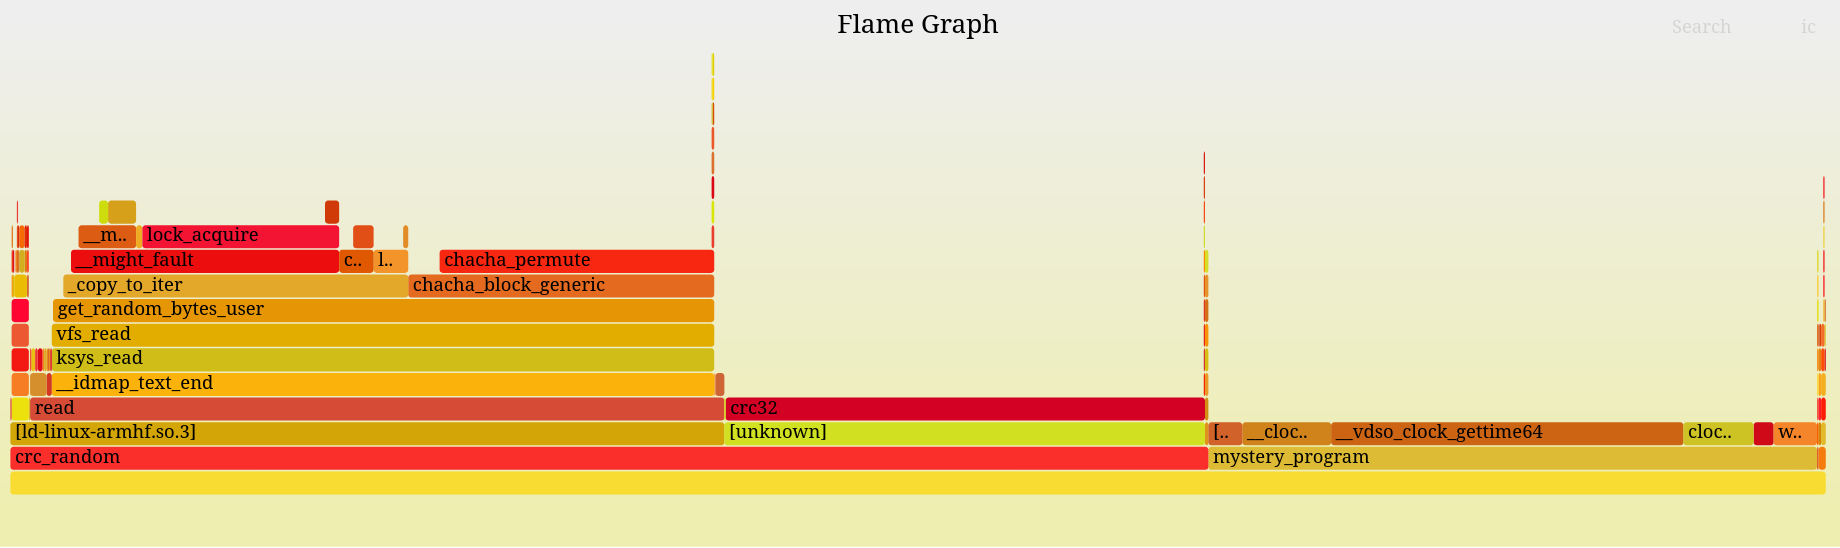
\includegraphics[width=1.0\textwidth]{slides/debugging-system-wide-profiling/flamegraph.png}\\
  \begin{itemize}
    \item The plates on top represent the functions sampled by perf during
      the recording
    \item The plates width represents how often a function has been
      sampled by perf
    \item The plates below represent the call stacks for the sampled functions
    \item Flamegraphs are interactive: clicking on a plate will zoom on the
      corresponding callstack
    \item Colors can be tuned at flamegraph generation (eg: to get a clear
      split between kernel and userspace)
  \end{itemize}
\end{frame}

\begin{frame}[fragile]
  \frametitle{Visualizing data with hotspot (1/2)}
  \begin{itemize}
	  \item Designed to provide a frontend to perf data files
    \item Can generate flamegraphs on the fly, but not only:
      \begin{itemize}
        \item CPU/tasks timelines
        \item Interactive callstacks navigation
        \item Code disassembly
      \end{itemize}
    \item Configurable (eg: allows to set paths to find all needed debug
      informations)
  \end{itemize}
\end{frame}

\begin{frame}[fragile]
  \frametitle{Visualizing data with hotspot (2/2)}
  \center 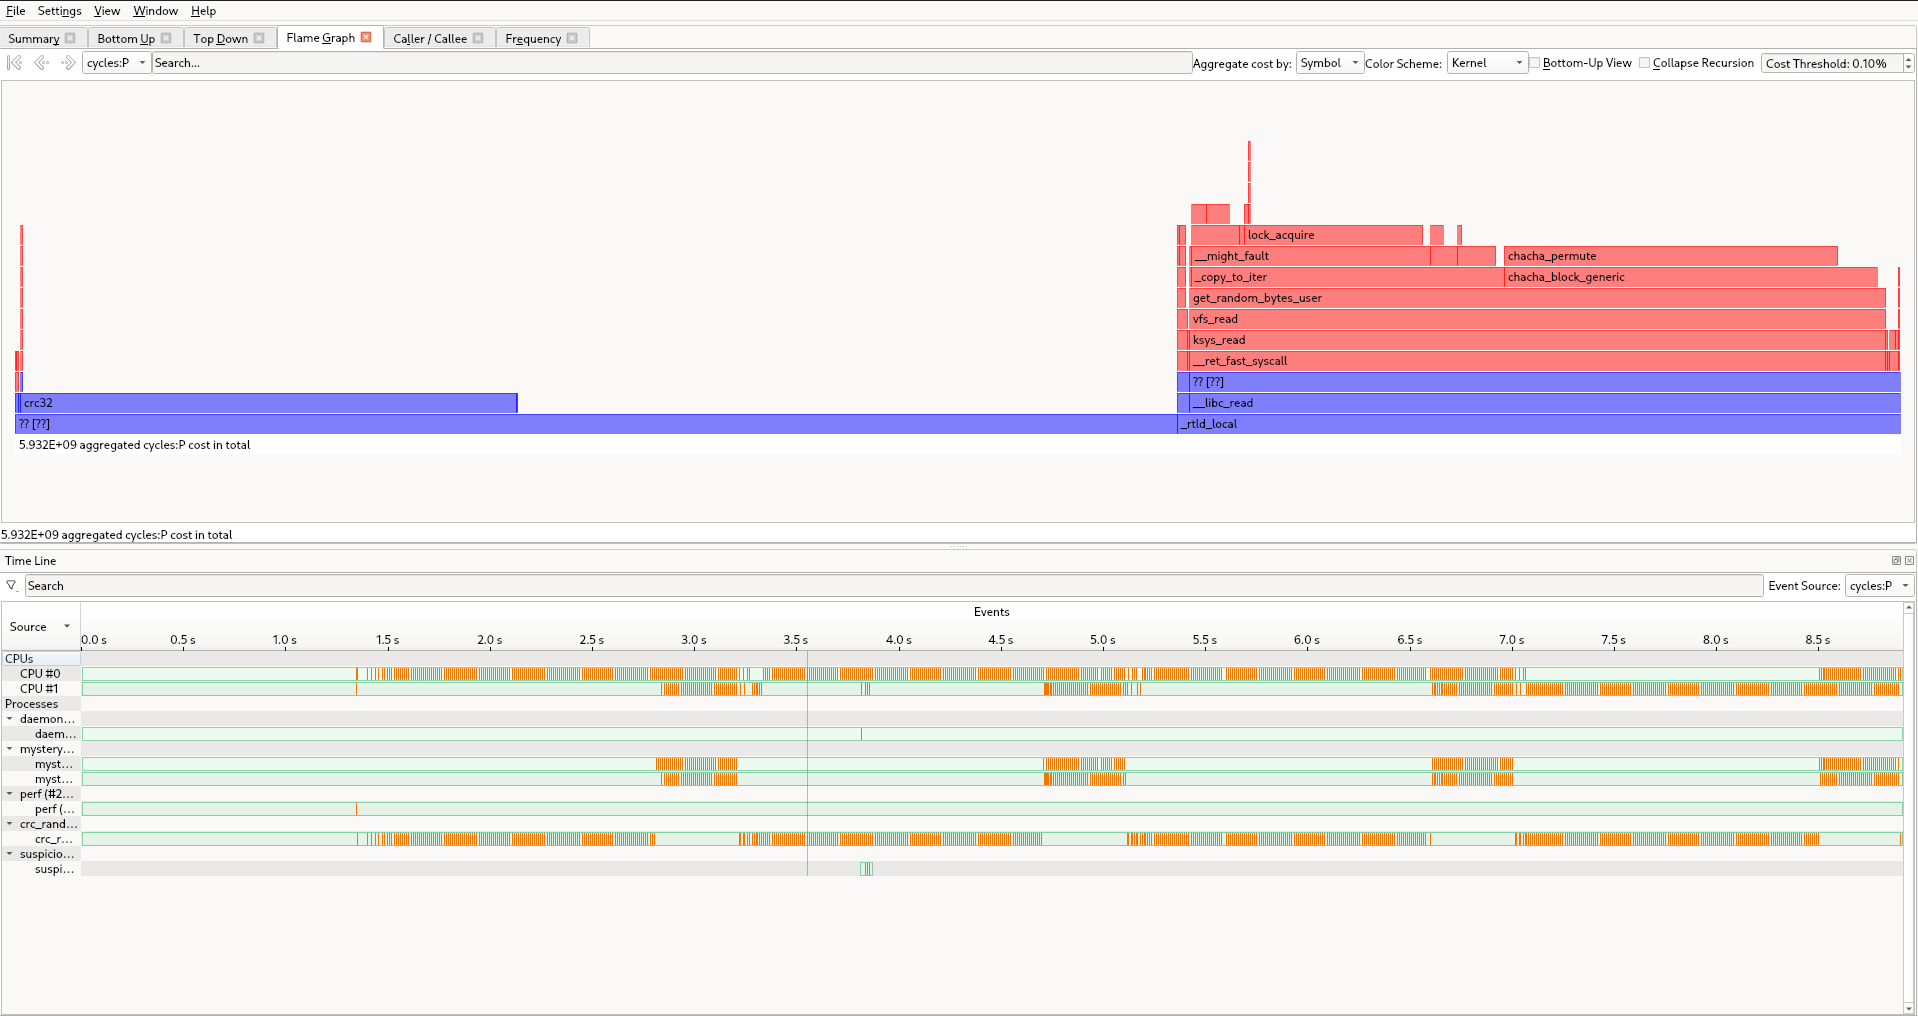
\includegraphics[width=0.9\textwidth]{slides/debugging-system-wide-profiling/hotspot.png}\\
\end{frame}

\subsection{ftrace and trace-cmd}

\begin{frame}
  \frametitle{ftrace}
  \begin{itemize}
    \item {\em ftrace} is a tracing framework within the kernel which stands for
          "Function Tracer".
    \item It offers a wide range of tracing capabilities allowing to observe the
          system behavior.
    \begin{itemize}
      \item Trace static tracepoints already inserted at various locations
            in the kernel (scheduler, interrupts, etc).
      \item Relies on GCC mcount() capability and kernel code patching mechanism
            to call {\em ftrace} tracing handlers.
    \end{itemize}
    \item All traces are recorded in a ring buffer that is optimized for tracing.
    \item Uses {\em tracefs} filesystem to control and display tracing events.
    \begin{itemize}
      \item \codewithhash{\# mount -t tracefs nodev /sys/kernel/tracing}.
    \end{itemize}
    \item {\em ftrace} support must be enabled in the kernel using
          \kconfigval{CONFIG_FTRACE}{y}.
    \item \kconfig{CONFIG_DYNAMIC_FTRACE} allows to have a zero overhead tracing
          support.
  \end{itemize}
\end{frame}

\begin{frame}
  \frametitle{ftrace files}
  \begin{itemize}
    \item {\em ftrace} controls are exposed through some specific files located under
          \code{/sys/kernel/tracing}.
    \begin{itemize}
      \item \code{current_tracer}: Current tracer that is used.
      \item \code{available_tracers}: List of available tracers that are
            compiled in the kernel.
      \item \code{tracing_on}: Enable/disable tracing.
      \item \code{trace}: Acquired trace in human readable format. Format will
            differ depending on the tracer used.
      \item \code{trace_pipe}: same as \code{trace}, but each read consumes the
      trace as it is read.
      \item \code{trace_marker{_raw}}: Emit comments from userspace in the
            trace buffer.
      \item \code{set_ftrace_filter}: Filter some specific functions.
      \item \code{set_graph_function}: Graph only the specified functions child.
    \end{itemize}
    \item Many other files are exposed, see \kdochtml{trace/ftrace}.
    \item {\em trace-cmd} CLI and {\em Kernelshark} GUI tools allow to record
          and visualize tracing data more easily.
  \end{itemize}
\end{frame}

\begin{frame}[fragile]
  \frametitle{ftrace tracers}
  \begin{itemize}
    \item ftrace provides several "tracers" which allow to trace different things.
    \item The tracer to be used should be written to the \code{current_tracer} file
    \begin{itemize}
      \item \code{nop}: Trace nothing, used to disable all tracing.
      \item \code{function}: Trace all kernel functions that are called.
      \item \code{function_graph}: Similar to \code{function} but traces both entry and exit.
      \item \code{hwlat}: Trace hardware latency.
      \item \code{irqsoff}: Trace sections where interrupts are disabled.
      \item \code{branch}: Trace likely()/unlikely() prediction errors.
      \item \code{mmiotrace}: Trace all accesses to the hardware (\code{read[bwlq]/write[bwlq]}).
    \end{itemize}
    \item \textbf{Warning: Some tracers can be expensive!}
  \end{itemize}
  \begin{block}{}
    \begin{minted}[fontsize=\small]{console}
# echo "function" > /sys/kernel/tracing/current_tracer
    \end{minted}
  \end{block}
\end{frame}

\begin{frame}[fragile]
  \frametitle{function\_graph tracer report example}
  \begin{itemize}
    \item The {\em function\_graph} traces all the function that
      executed and their associated callgraphs
    \item Will display the process, CPU, timestamp and function graph:
  \end{itemize}
  \begin{block}{}
    \begin{minted}[fontsize=\tiny]{console}
$ trace-cmd report
...
dd-113   [000]   304.526590: funcgraph_entry:                   |  sys_write() {
dd-113   [000]   304.526597: funcgraph_entry:                   |    ksys_write() {
dd-113   [000]   304.526603: funcgraph_entry:                   |      __fdget_pos() {
dd-113   [000]   304.526609: funcgraph_entry:        6.541 us   |        __fget_light();
dd-113   [000]   304.526621: funcgraph_exit:       + 18.500 us  |      }
dd-113   [000]   304.526627: funcgraph_entry:                   |      vfs_write() {
dd-113   [000]   304.526634: funcgraph_entry:        6.334 us   |        rw_verify_area();
dd-113   [000]   304.526646: funcgraph_entry:        6.208 us   |        write_null();
dd-113   [000]   304.526658: funcgraph_entry:        6.292 us   |        __fsnotify_parent();
dd-113   [000]   304.526669: funcgraph_exit:       + 43.042 us  |      }
dd-113   [000]   304.526675: funcgraph_exit:       + 78.833 us  |    }
dd-113   [000]   304.526680: funcgraph_exit:       + 91.291 us  |  }
dd-113   [000]   304.526689: funcgraph_entry:                   |  sys_read() {
dd-113   [000]   304.526695: funcgraph_entry:                   |    ksys_read() {
dd-113   [000]   304.526702: funcgraph_entry:                   |      __fdget_pos() {
dd-113   [000]   304.526708: funcgraph_entry:        6.167 us   |        __fget_light();
dd-113   [000]   304.526719: funcgraph_exit:       + 18.083 us  |      }
    \end{minted}
  \end{block}
\end{frame}

\begin{frame}
  \frametitle{irqsoff tracer}
  \begin{itemize}
    \item ftrace {\em irqsoff} tracer allows to trace the irqs latency due to
          interrupts being disabled for too long.
    \item Helpful to find why interrupts have high latencies on a system.
    \item This tracer will record the longest trace with interrupts being disabled.
    \item This tracer needs to be enabled with \kconfigval{IRQSOFF_TRACER}{y}.
    \begin{itemize}
      \item \code{preemptoff}, \code{premptirqsoff} tracers also exist to trace
            section of code were preemption is disabled.
    \end{itemize}
  \end{itemize}
  \center\includegraphics[height=0.3\textheight]{slides/debugging-system-wide-profiling/kernel_irqsoff.pdf}
\end{frame}

\begin{frame}[fragile]
  \frametitle{irqsoff: report example}
  \begin{block}{}
    \begin{minted}[fontsize=\tiny]{console}
# latency: 276 us, #104/104, CPU#0 | (M:preempt VP:0, KP:0, SP:0 HP:0 #P:2)
#    -----------------
#    | task: stress-ng-114 (uid:0 nice:0 policy:0 rt_prio:0)
#    -----------------
#  => started at: __irq_usr
#  => ended at:   irq_exit
#
#
#                    _------=> CPU#            
#                   / _-----=> irqs-off        
#                  | / _----=> need-resched    
#                  || / _---=> hardirq/softirq 
#                  ||| / _--=> preempt-depth   
#                  |||| /     delay            
#  cmd     pid     ||||| time  |   caller      
#     \   /        |||||  \    |   /         
stress-n-114       0d...    2us : __irq_usr
stress-n-114       0d...    7us : gic_handle_irq <-__irq_usr
stress-n-114       0d...   10us : __handle_domain_irq <-gic_handle_irq
...
stress-n-114       0d...  270us : __local_bh_disable_ip <-__do_softirq
stress-n-114       0d.s.  275us : __do_softirq <-irq_exit
stress-n-114       0d.s.  279us+: tracer_hardirqs_on <-irq_exit
stress-n-114       0d.s.  290us : <stack trace>
    \end{minted}
  \end{block}
\end{frame}

\begin{frame}
  \frametitle{Hardware latency detector}
  \begin{itemize}
    \item ftrace {\em hwlat} tracer will help to find if the hardware generates
          latency.
    \begin{itemize}
      \item Sytem Management interrupts for instance are non maskable and
            directly trigger some firmware support feature, suspending CPU execution.
      \item Interrupts handled by secure monitor can also cause this kind of
            latency.
    \end{itemize}
    \item If some latency is found with this tracer, the system is probably
          not suitable for real time usage.
    \item Uses a single core looping while interrupts are disabled and measuring
          the time elapsed between two consecutive time reads.
    \item Needs to be builtin the kernel with \kconfigval{CONFIG_HWLAT_TRACER}{y}.
  \end{itemize}

  \center\includegraphics[height=0.25\textheight]{slides/debugging-system-wide-profiling/kernel_hwlat.pdf}
\end{frame}

\begin{frame}
  \frametitle{trace-cmd}
  \begin{itemize}
    \item {\em trace-cmd} is a tool written by Steven Rostedt which allows
          interacting with {\em ftrace} (\manpage{trace-cmd}{1}).
    \item The tracers supported by {\em trace-cmd} are those exposed by ftrace.
    \item {\em trace-cmd} offers multiple commands:
    \begin{itemize}
      \item {\em list}: List available plugins/events that can be recorded.
      \item {\em record}: Record a trace into the file \code{trace.dat}.
      \item {\em report}: Display \code{trace.dat} acquisition results.
    \end{itemize}
    \item At the end of recording, a \code{trace.dat} file will be generated.
  \end{itemize}
\end{frame}

\begin{frame}[fragile]
  \frametitle{trace-cmd examples (1/3)}
  \begin{itemize}
    \item List available tracers
  \end{itemize}
  \begin{block}{}
    \begin{minted}[fontsize=\tiny]{console}
$ trace-cmd list -t
blk mmiotrace function_graph function nop
    \end{minted}
  \end{block}
  \begin{itemize}
    \item List available events
  \end{itemize}
  \begin{block}{}
    \begin{minted}[fontsize=\tiny]{console}
$ trace-cmd list -e
...
migrate:mm_migrate_pages_start
migrate:mm_migrate_pages
tlb:tlb_flush
syscalls:sys_exit_process_vm_writev
...
    \end{minted}
  \end{block}
  
  \begin{itemize}
    \item List available functions for filtering with \code{function} and
        \code{function_graph} tracers
  \end{itemize}
  \begin{block}{}
    \begin{minted}[fontsize=\tiny]{console}
$ trace-cmd list -f
...
wait_for_initramfs
__ftrace_invalid_address___64
calibration_delay_done
calibrate_delay
...
    \end{minted}
  \end{block}
\end{frame}

\begin{frame}[fragile]
  \frametitle{trace-cmd examples (2/3)}
  \begin{itemize}
    \item Start the function tracer and record data globally on the system
  \end{itemize}
  \begin{block}{}
    \begin{minted}[fontsize=\tiny]{console}
$ trace-cmd record -p function
    \end{minted}
  \end{block}

  \begin{itemize}
    \item Use the function graph tracer but filter only \code{spi_*} functions
  \end{itemize}
  \begin{block}{}
    \begin{minted}[fontsize=\tiny]{console}
$ trace-cmd record -l spi_* -p function_graph
    \end{minted}
  \end{block}

  \begin{itemize}
    \item Run the {\em irqsoff} tracer on the system:
  \end{itemize}
  \begin{block}{}
    \begin{minted}[fontsize=\tiny]{console}
$ trace-cmd record -p irqsoff
    \end{minted}
  \end{block}
  \begin{itemize}
    \item Record only \code{irq_handler_exit/irq_handler_entry} events on the
          system:
  \end{itemize}
  \begin{block}{}
    \begin{minted}[fontsize=\tiny]{console}
$ trace-cmd record -e irq:irq_handler_exit -e irq:irq_handler_entry
    \end{minted}
  \end{block}
\end{frame}

\begin{frame}[fragile]
  \frametitle{trace-cmd examples (3/3)}
  \begin{itemize}
    \item Visualize the data that have been acquired in \code{trace.dat}:
  \end{itemize}
  \begin{block}{}
    \begin{minted}[fontsize=\tiny]{console}
$ trace-cmd report
    \end{minted}
  \end{block}
  \begin{itemize}
    \item Reset all the {\em ftrace} buffers and remove tracers
  \end{itemize}
  \begin{block}{}
    \begin{minted}[fontsize=\tiny]{console}
$ trace-cmd reset
    \end{minted}
  \end{block}

\end{frame}

\begin{frame}
  \frametitle{Remote tracing with trace-cmd}
  \begin{itemize}
    \item {\em trace-cmd} output can be quite big and thus difficult to
          store on an embedded platform with limited storage.
    \item For that purpose, a \code{listen} command is available and allows sending
          the acquisitions over the network:
    \begin{itemize}
      \item Run \code{trace-cmd listen -p 6578} on the remote system that will
            be collecting the traces
      \item On the target system, use \code{trace-cmd record -N <target_ip>:6578}
            to specify the remote system that will collect the traces
    \end{itemize}
  \end{itemize}
  \center\includegraphics[height=0.15\textheight]{slides/debugging-system-wide-profiling/ftrace-remote.pdf}
\end{frame}

\begin{frame}[fragile]
  \frametitle{\kfunc{trace_printk}}
  \begin{itemize}
    \item \kfunc{trace_printk} allows to emit strings in the trace buffer
    \item Useful to trace some specific conditions in your code and display it in the trace buffer 
  \end{itemize}
  \begin{block}{}
    \begin{minted}[fontsize=\tiny]{C}
#include <linux/ftrace.h>
void read_hw()
{
  if (condition)
    trace_printk("Condition is true!\n");
}
    \end{minted}
  \end{block}
  \begin{itemize}
    \item Will display the following in the trace buffer for \code{function_graph} tracer
  \end{itemize}
  \begin{block}{}
    \begin{minted}[fontsize=\tiny]{console}
1)               |             read_hw() {
1)               |                /* Condition is true! */
1)   2.657 us    |             }
    \end{minted}
  \end{block}
\end{frame}

\begin{frame}[fragile]
  \frametitle{Adding ftrace tracepoints (1/2)}
  \begin{itemize}
    \item For some custom needs, it might be needed to add custom tracepoints
    \item First, one needs to declare the tracepoint definition in a \code{.h}
          file
  \end{itemize}
  \begin{block}{}
    \begin{minted}[fontsize=\footnotesize]{C}
#undef TRACE_SYSTEM
#define TRACE_SYSTEM subsys

#if !defined(_TRACE_SUBSYS_H) || defined(TRACE_HEADER_MULTI_READ)
#define _TRACE_SUBSYS_H

#include <linux/tracepoint.h>

DECLARE_TRACE(subsys_eventname,
        TP_PROTO(int firstarg, struct task_struct *p),
        TP_ARGS(firstarg, p));

#endif /* _TRACE_SUBSYS_H */

/* This part must be outside protection */
#include <trace/define_trace.h>
    \end{minted}
  \end{block}
\end{frame}

\begin{frame}[fragile]
  \frametitle{Adding ftrace tracepoints (2/2)}
  \begin{itemize}
    \item Then, emit tracepoint in a \code{.c} file using that header file
  \end{itemize}
  \begin{block}{}
    \begin{minted}[fontsize=\footnotesize]{C}
#include <trace/events/subsys.h>

#define CREATE_TRACE_POINTS
DEFINE_TRACE(subsys_eventname);

void any_func(void)
{
  ...
  trace_subsys_eventname(arg, task);
  ...
}
    \end{minted}
  \end{block}
  \begin{itemize}
    \item See \kdochtml{trace/tracepoints} for more information
  \end{itemize}
\end{frame}

\begin{frame}[fragile]
  \frametitle{Kernelshark}
  \begin{columns}
    \column{0.65\textwidth}
    \begin{itemize}
      \item Kernelshark is a Qt-based graphical interface for processing
            {\em trace-cmd} trace.dat reports.
      \item Can also setup and acquire data using {\em trace-cmd}.
      \item Displays CPU and tasks as different colors along with the recorded
            events.
      \item Useful when a deep analysis is required for a specific bug.
    \end{itemize}
    \column{0.35\textwidth}
    \vspace{0.5cm}
    \center\includegraphics[height=0.6\textheight]{slides/debugging-system-wide-profiling/kernelshark-logo.png}
  \end{columns}
\end{frame}

\begin{frame}
  \frametitle{kernelshark}
  \center\includegraphics[height=0.8\textheight]{slides/debugging-system-wide-profiling/kernelshark.png}
\end{frame}

\setuplabframe
{System wide profiling}
{
  Profiling a system from userspace to kernel space
  \begin{itemize}
    \item Profiling with ftrace, uprobes and kernelshark
    \item Profiling with perf
  \end{itemize}
}

\subsection{LTTng}

\begin{frame}
  \frametitle{LTTng}
  \begin{columns}
    \column{0.65\textwidth}
    \begin{itemize}
      \item LTTng is an open source tracing framework for Linux maintained by
            the \href{https://www.efficios.com/}{EfficiOS} company.
      \item LTTng allows understanding the interactions between the kernel and
            applications (C, C++, Java, Python).
      \begin{itemize}
        \item Also expose a \code{/dev/lttng-logger} that can be used from any
              application.
      \end{itemize}
      \item Tracepoints are associated with a payload (data).
      \item LTTng is focused on low-overhead tracing.
      \item Uses the Common Trace Format (so traces are readable with other
      software like babeltrace or trace-compass)
    \end{itemize}
    \column{0.35\textwidth}
    \includegraphics[height=0.3\textheight]{slides/debugging-system-wide-profiling/lttng-logo.jpg}
  \end{columns}
\end{frame}

\begin{frame}
  \frametitle{Tracepoints with LTTng}
  \begin{itemize}
    \item LTTng works with a session daemon that receive all events from kernel
          and userspace LTTng tracing components.
    \item LTTng can use and trace the following instrumentation points:
    \begin{itemize}
      \item LTTng kernel tracepoints
      \item kprobes and kretprobes
      \item Linux kernel system calls
      \item Linux user space probe
      \item User space LTTng tracepoints
    \end{itemize}
  \end{itemize}
\end{frame}

\begin{frame}
  \frametitle{Creating userspace tracepoints with LTTng}
  \begin{itemize}
    \item New userspace tracepoints can be defined using LTTng.
    \item Tracepoints have multiple characteristics:
    \begin{itemize}
      \item A provider namespace
      \item A name identifying the tracepoint
      \item Parameters of various types (int, char *, etc)
      \item Fields describing how to display the tracepoint parameters
            (decimal, hexadecimal, etc) (see \href{https://lttng.org/man/3/lttng-ust/v2.13/}{LTTng-ust} manpage
            for types)
    \end{itemize}
    \item Developers must perform multiple operations to use UST tracepoint:
    write a tracepoint provider (.h), write a tracepoint package (.c), build
    the package, call the tracepoint in the traced application, and finally
    build the application, linked with lttng-ust library and the package provider.
    \item LTTng provides the \code{lttng-gen-tp} to ease all those steps,
    allowing to only write a template (.tp) file.
  \end{itemize}
\end{frame}

\begin{frame}[fragile]
  \frametitle{Defining a LTTng tracepoint (1/2)}

  \begin{itemize}
    \item Tracepoint template (\code{hello_world-tp.tp}):
    \begin{block}{}
      \begin{minted}[fontsize=\tiny]{C}
    LTTNG_UST_TRACEPOINT_EVENT(
      // Tracepoint provider name
      hello_world,

      // Tracepoint/event name
      my_first_tracepoint,

      // Tracepoint arguments (input)
      LTTNG_UST_TP_ARGS(
          char *, text
      ),

      // Tracepoint/event fields (output)
      LTTNG_UST_TP_FIELDS(
          lttng_ust_field_string(message, text)
      )
    )
     \end{minted}
    \end{block}
    \item \code{lttng-gen-tp} will take this template file and generate/build
    all needed files (.h, .c and .o files)
  \end{itemize}
\end{frame}

\begin{frame}[fragile]
  \frametitle{Defining a LTTng tracepoint (2/2)}
  \begin{itemize}
    \item Build tracepoint provider:
  \end{itemize}
  \begin{block}{}
    \begin{minted}[fontsize=\tiny]{console}
$ lttng-gen-tp hello_world-tp.tp
   \end{minted}
  \end{block}
  \begin{itemize}
    \item Tracepoint usage (\code{hello_world.c}):
  \end{itemize}
  \begin{block}{}
    \begin{minted}[fontsize=\tiny]{C}
#include <stdio.h>
#include "hello-tp.h"

int main(int argc, char *argv[])
{
    lttng_ust_tracepoint(hello_world, my_first_tracepoint, "hi there!");
    return 0;
}
   \end{minted}
  \end{block}
  \begin{itemize}
    \item Compilation:
  \end{itemize}
  \begin{block}{}
    \begin{minted}[fontsize=\tiny]{console}
$ gcc hello_world.c hello_world-tp.o -llttng-ust -o hello_world
   \end{minted}
  \end{block}
\end{frame}

\begin{frame}[fragile]
  \frametitle{Using LTTng}
  \begin{block}{}
    \begin{minted}[fontsize=\small]{console}
$ lttng create my-tracing-session --output=./my_traces
$ lttng list --kernel
$ lttng list --userspace
$ lttng enable-event --userspace hello_world:my_first_tracepoint
$ lttng enable-event --kernel --syscall open,close,write
$ lttng start
$ /* Run your application or do something */
$ lttng destroy
$ babeltrace2 ./my_traces
   \end{minted}
  \end{block}
  \begin{itemize}
    \item You can also use
    \href{https://eclipse.dev/tracecompass/trace-compass}{trace-compass}
    to display the traces in a GUI
  \end{itemize}
\end{frame}

\begin{frame}[fragile]
  \frametitle{Remote tracing with LTTng}
  \begin{itemize}
    \item LTTng allows to record traces over the network.
    \item Useful for embedded systems with limited storage capabilities.
    \item On the remote computer, run \code{lttng-relayd} command
  \end{itemize}
  \begin{block}{}
    \begin{minted}[fontsize=\small]{console}
$ lttng-relayd --output=${PWD}/traces
   \end{minted}
  \end{block}
  \begin{itemize}
    \item Then on the target, at session creation, use the \code{--set-url}
  \end{itemize}
  \begin{block}{}
    \begin{minted}[fontsize=\small]{console}
$ lttng create my-session --set-url=net://remote-system
   \end{minted}
  \end{block}
  \begin{itemize}
    \item Traces will then be recorded directly on the remote computer.
  \end{itemize}
\end{frame}

\subsection{eBPF}

\begin{frame}{The ancestor: Berkeley Packet filter}
  \begin{itemize}
    \item BPF stands for Berkeley Packet Filter and was initially used
    for network packet filtering
    \item BPF is implemented and used in Linux to perform Linux Socket
    Filtering (see \kdochtml{networking/filter})
    \item tcpdump and Wireshark heavily rely on BPF (through libpcap) for
    packet capture
  \end{itemize}
\end{frame}

\begin{frame}{BPF in libpcap: setup}
  \begin{columns}
    \column{0.75\textwidth}
    \begin{itemize}
    \item tcpdump passes the capture filter string from the user to libpcap
    \item libpcap translates the capture filter into a binary program
      \begin{itemize}
      \item This program uses the instruction set of an abstract machine
        (the ``BPF instruction set'')
      \end{itemize}
    \item libpcap sends the binary program to the kernel via the
      \code{setsockopt()} syscall
    \end{itemize}
    \column{0.25\textwidth}
      \includegraphics[height=0.85\textheight]{slides/debugging-system-wide-profiling/bpf-setup.pdf}
  \end{columns}
\end{frame}

\begin{frame}{BPF in libpcap: capture}
  \begin{columns}
    \column{0.55\textwidth}
    \begin{itemize}
    \item The kernel implements the BPF ``virtual machine''
    \item The BPF virtual machine executes the program for every packet
    \item The program inspects the packet data and returns a non-zero value
      if the packet must be captured
    \item If the return value is non-zero, the packet is captured in
      addition to regular packet processing
    \end{itemize}
    \column{0.45\textwidth}
      \includegraphics[height=0.80\textheight]{slides/debugging-system-wide-profiling/bpf-capture.pdf}
  \end{columns}
\end{frame}

\begin{frame}
  \frametitle{eBPF (1/2)}
  \begin{itemize}
    \item \href{https://ebpf.io/}{eBPF} is a new framework allowing to run
    small user programs directly in the kernel, in a safe and efficient way. It
    has been added in kernel 3.18 but it is still evolving and receiving
    updates frequently.
    \item eBPF programs can capture and expose kernel data to userspace, and
    also alter kernel behavior based on some user-defined rules.
    \item eBPF is event-driven: an eBPF program is triggered and executed on a
    specific kernel event
    \item A major benefit from eBPF is the possibility to reprogram the kernel
    behavior, without performing kernel development:
    \begin{itemize}
      \item no risk of crashing the kernel because of bugs
      \item faster development cycles to get a new feature ready
    \end{itemize}
  \end{itemize}
  \center
\includegraphics[height=0.2\textheight]{slides/debugging-linux-application-stack/logo_ebpf.png}\\
  \tiny Image credits: \url{https://ebpf.io/}
\end{frame}

\begin{frame}
  \frametitle{eBPF (2/2)}
  \begin{itemize}
    \item The most notable eBPF features are:
    \begin{itemize}
      \item A new instruction set, interpreter and verifier
      \item A wide variety of "attach" locations, allowing to hook programs
      almost anywhere in the kernel
      \item dedicated data structures called "maps", to exchange data between
      multiple eBPF programs or between programs and userspace
      \item A dedicated \code{bpf()} syscall to manipulate eBPF programs and data
      \item plenty of (kernel) helper functions accessible from eBPF programs.
    \end{itemize}
  \end{itemize}
\end{frame}

\begin{frame}
  \frametitle{eBPF program lifecycle}
  \begin{center}
    \includegraphics[height=0.8\textheight]{slides/debugging-system-wide-profiling/bpf_lifecycle.pdf}
  \end{center}
\end{frame}

\begin{frame}[fragile]
  \frametitle{Kernel configuration for eBPF}
  \begin{itemize}
    \item \kconfig{CONFIG_NET} to enable eBPF subsystem
    \item \kconfig{CONFIG_BPF_SYSCALL} to enable the \code{bpf()} syscall
    \item \kconfig{CONFIG_BPF_JIT} to enable JIT on programs and so increase performance
    \item \kconfig{CONFIG_BPF_JIT_ALWAYS_ON} to force JIT
    \item \kconfigval{CONFIG_BPF_UNPRIV_DEFAULT_OFF}{n} in \textbf{development} to
    allow eBPF usage without root
    \item You may then want to enable more general features to "unlock"
    specific hooking locations:
    \begin{itemize}
      \item \kconfig{CONFIG_KPROBES} to allow hooking programs on kprobes
      \item \kconfig{CONFIG_TRACING} to allow hooking programs on kernel tracepoints
      \item \kconfig{CONFIG_NET_CLS_BPF} to write packets classifiers
      \item \kconfig{CONFIG_CGROUP_BPF} to attach programs on cgroups hooks
    \end{itemize}
  \end{itemize}
\end{frame}

\begin{frame}[fragile]
  \frametitle{eBPF ISA}
  \begin{itemize}
    \item eBPF is a "virtual" ISA, defining its own set of instructions: load
    and store instructions, arithmetic instructions, jump instructions,etc
    \item It also defines a set of 10 64-bits wide registers as well as a
    calling convention:
    \begin{itemize}
      \item \code{R0}: return value from functions and BPF program
      \item \code{R1, R2, R3, R4, R5}: function arguments
      \item \code{R6, R7, R8, R9}: callee-saved registers
      \item \code{R10}: stack pointer
    \end{itemize}
  \end{itemize}
  \begin{block}{}
    \begin{minted}[fontsize=\scriptsize]{console}
; bpf_printk("Hello %s\n", "World");
      0:  r1 = 0x0 ll
      2:  r2 = 0xa
      3:  r3 = 0x0 ll
      5:  call 0x6
; return 0;
      6:  r0 = 0x0
      7:  exit
    \end{minted}
  \end{block}
\end{frame}

\begin{frame}[fragile]
  \frametitle{The eBPF verifier}
  \begin{itemize}
    \item When loaded into the kernel, a program must first be validated by the
    eBPF verifier.
    \item The verifier is a complex piece of software which checks eBPF
    programs against a set of rules to ensure that running those may not
    compromise the whole kernel. For example:
    \begin{itemize}
      \item a program must always return and so not contain paths which could
      make them "infinite" (e.g: no infinite loop)
      \item a program must make sure that a pointer is valid before
      dereferencing it
      \item a program cannot access arbitrary memory addresses, it must use
      passed context and available helpers
    \end{itemize}
    \item If a program violates one of the verifier rules, it will be rejected.
    \item Despite the presence of the verifier, you still need to be careful when
    writing programs! eBPF programs run with preemption enabled (but CPU
    migration disabled), so they can still suffer from concurrency issues
    \begin{itemize}
      \item There are mechanisms and helpers to avoid those issues, like
        per-CPU maps types.
    \end{itemize}
  \end{itemize}
\end{frame}

\begin{frame}[fragile]
  \frametitle{Program types and attach points}
  \begin{itemize}
    \item There are different categories of hooks to which a program can be
    attached:
    \begin{itemize}
      \item an arbitrary kprobe
      \item a kernel-defined static tracepoint
      \item a specific perf event
      \item throughout the network stack
      \item an arbitrary uprobe
      \item and a lot more, see \ksym{bpf_attach_type}
    \end{itemize}
    \item A specific attach-point type can only be hooked with a set of
    specific program types, see \ksym{bpf_prog_type} and
    \kdochtml{bpf/libbpf/program_types}.
    \item The program type then defines the data passed to an eBPF program as
    input when it is invoked. For example:
    \begin{itemize}
      \item A \code{BPF_PROG_TYPE_TRACEPOINT} program will receive a structure
      containing all data returned to userspace by the targeted tracepoint.
      \item A \code{BPF_PROG_TYPE_SCHED_CLS} program (used to implement packet
      classifiers) will receive a \kstruct{__sk_buff}, the kernel
      representation of a socket buffer.
      \item You can learn about the context passed to any program type by
      checking \kfile{include/linux/bpf_types.h}
    \end{itemize}
  \end{itemize}
\end{frame}

\begin{frame}[fragile]
  \frametitle{eBPF maps}
  \begin{itemize}
    \item eBPF programs exchange data with userspace or other programs through
    maps of different natures:
    \begin{itemize}
      \item \code{BPF_MAP_TYPE_ARRAY}: generic array storage. Can be
      differentiated per CPU
      \item \code{BPF_MAP_TYPE_HASH}: a storage composed of key-value pairs.
      Keys can be of different types: \code{__u32}, a device type, an IP address...
      \item \code{BPF_MAP_TYPE_QUEUE}: a FIFO-type queue
      \item \code{BPF_MAP_TYPE_CGROUP_STORAGE}: a specific hash map keyed by a
      cgroup id. There are other types of maps specific to other object types
      (inodes, tasks, sockets, etc)
      \item etc...
    \end{itemize}
    \item For basic data, it is easier and more efficient to directly use eBPF
    global variables (no syscalls involved, contrary to maps)
  \end{itemize}
\end{frame}

\begin{frame}[fragile]
  \frametitle{The \code{bpf()} syscall}
  \begin{itemize}
    \item The kernel exposes a \code{bpf()} syscall to allow interacting with the
    eBPF subsystem
    \item The syscall takes a set of subcommands, and depending on the
    subcommand, some specific data:
    \begin{itemize}
      \item \ksym{BPF_PROG_LOAD} to load a bpf program
      \item \ksym{BPF_MAP_CREATE} to allocate maps to be used by a program
      \item \ksym{BPF_MAP_LOOKUP_ELEM} to search for an entry in a map
      \item \ksym{BPF_MAP_UPDATE_ELEM} to update an entry in a map
      \item etc
    \end{itemize}
    \item The syscall works with file descriptors pointing to eBPF resources.
    Those resources (program, maps, links, etc) remain valid while there is at least
    one program holding a valid file descriptor to it. Those are automatically cleaned
    once there are no user left.
    \item For more details, see  \manpage{bpf}{2}
  \end{itemize}
\end{frame}

\begin{frame}[fragile]
  \frametitle{Writing eBPF programs}
  \begin{itemize}
    \item eBPF programs can either be written directly in raw eBPF assembly or in
    higher level languages (e.g: C or rust), and are compiled using the clang
    compiler.
    \item The kernel provides some helpers that can be called from an eBPF program:
    \begin{itemize}
      \item \code{bpf_trace_printk} Emits a log to the trace buffer
      \item \code{bpf_map_{lookup,update,delete}_elem} Manipulates maps
      \item \code{bpf_probe_{read,write}[_user]} Safely read/write data from/to kernel or userspace
      \item \code{bpf_get_current_pid_tgid} Returns current Process ID and Thread group ID
      \item \code{bpf_get_current_uid_gid} Returns current User ID and Group ID
      \item \code{bpf_get_current_comm} Returns the name of the executable running in the
      current task
      \item \code{bpf_get_current_task} Returns the current \kstruct{task_struct}
      \item Many other helpers are available, see \manpage{bpf-helpers}{7}
    \end{itemize}
    \item Kernel also exposes kfuncs (see \kdochtml{bpf/kfuncs}), but contrary
    to bpf-helpers, those do not belong to the kernel stable interface.
  \end{itemize}
\end{frame}

\begin{frame}[fragile]
  \frametitle{Manipulating eBPF program}
  \begin{itemize}
    \item There are different ways to build, load and manipulate eBPF programs:
    \begin{itemize}
      \item One way is to write an eBPF program, build it with clang, and then load it,
      attach it and read data from it with bare \code{bpf()} calls in a custom
      userspace program
      \item One can also use \code{bpftool} on the built ebpf program to
      manipulate it (load, attach, read maps, etc), without writing any userspace tool
      \item Or we can write our own eBPF tool thanks to some intermediate libraries which handle most of the
      hard work, like libbpf
      \item We can also use specialized frameworks like BCC or bpftrace to really
      get all operations (bpf program build included) handled
    \end{itemize}
  \end{itemize}
\end{frame}

\begin{frame}[fragile]
  \frametitle{BCC}
  \begin{columns}
    \column{0.75\textwidth}
    \begin{itemize}
      \item BPF Compiler Collection (BCC) is (as its name suggests) a collection
            of BPF based tools.
      \item BCC provides a large number of ready-to-use tools written in BPF.
      \item Also provides an interface to write, load and hook BPF programs more
            easily than using "raw" BPF language.
      \item Available on a large number of architectures and distributions
	      (but not packaged in Buildroot)
      \begin{itemize}
        \item On debian, when installed, all tools are named \code{<tool>-bpfcc}.
      \end{itemize}
      \item BCC requires a kernel version >= 4.1.
      \item BCC evolves quickly, many distributions have old versions: you
            may need to compile from the latest sources
    \end{itemize}
  \column{0.25\textwidth}
  \vspace{0.5cm}
  
\includegraphics[height=0.2\textheight]{slides/debugging-linux-application-stack/logo_bcc.png}\\
  \tiny Image credits: \url{https://github.com/iovisor/bcc}
  \end{columns}
\end{frame}

\begin{frame}[fragile]
  \frametitle{BCC tools}
  \begin{center}
    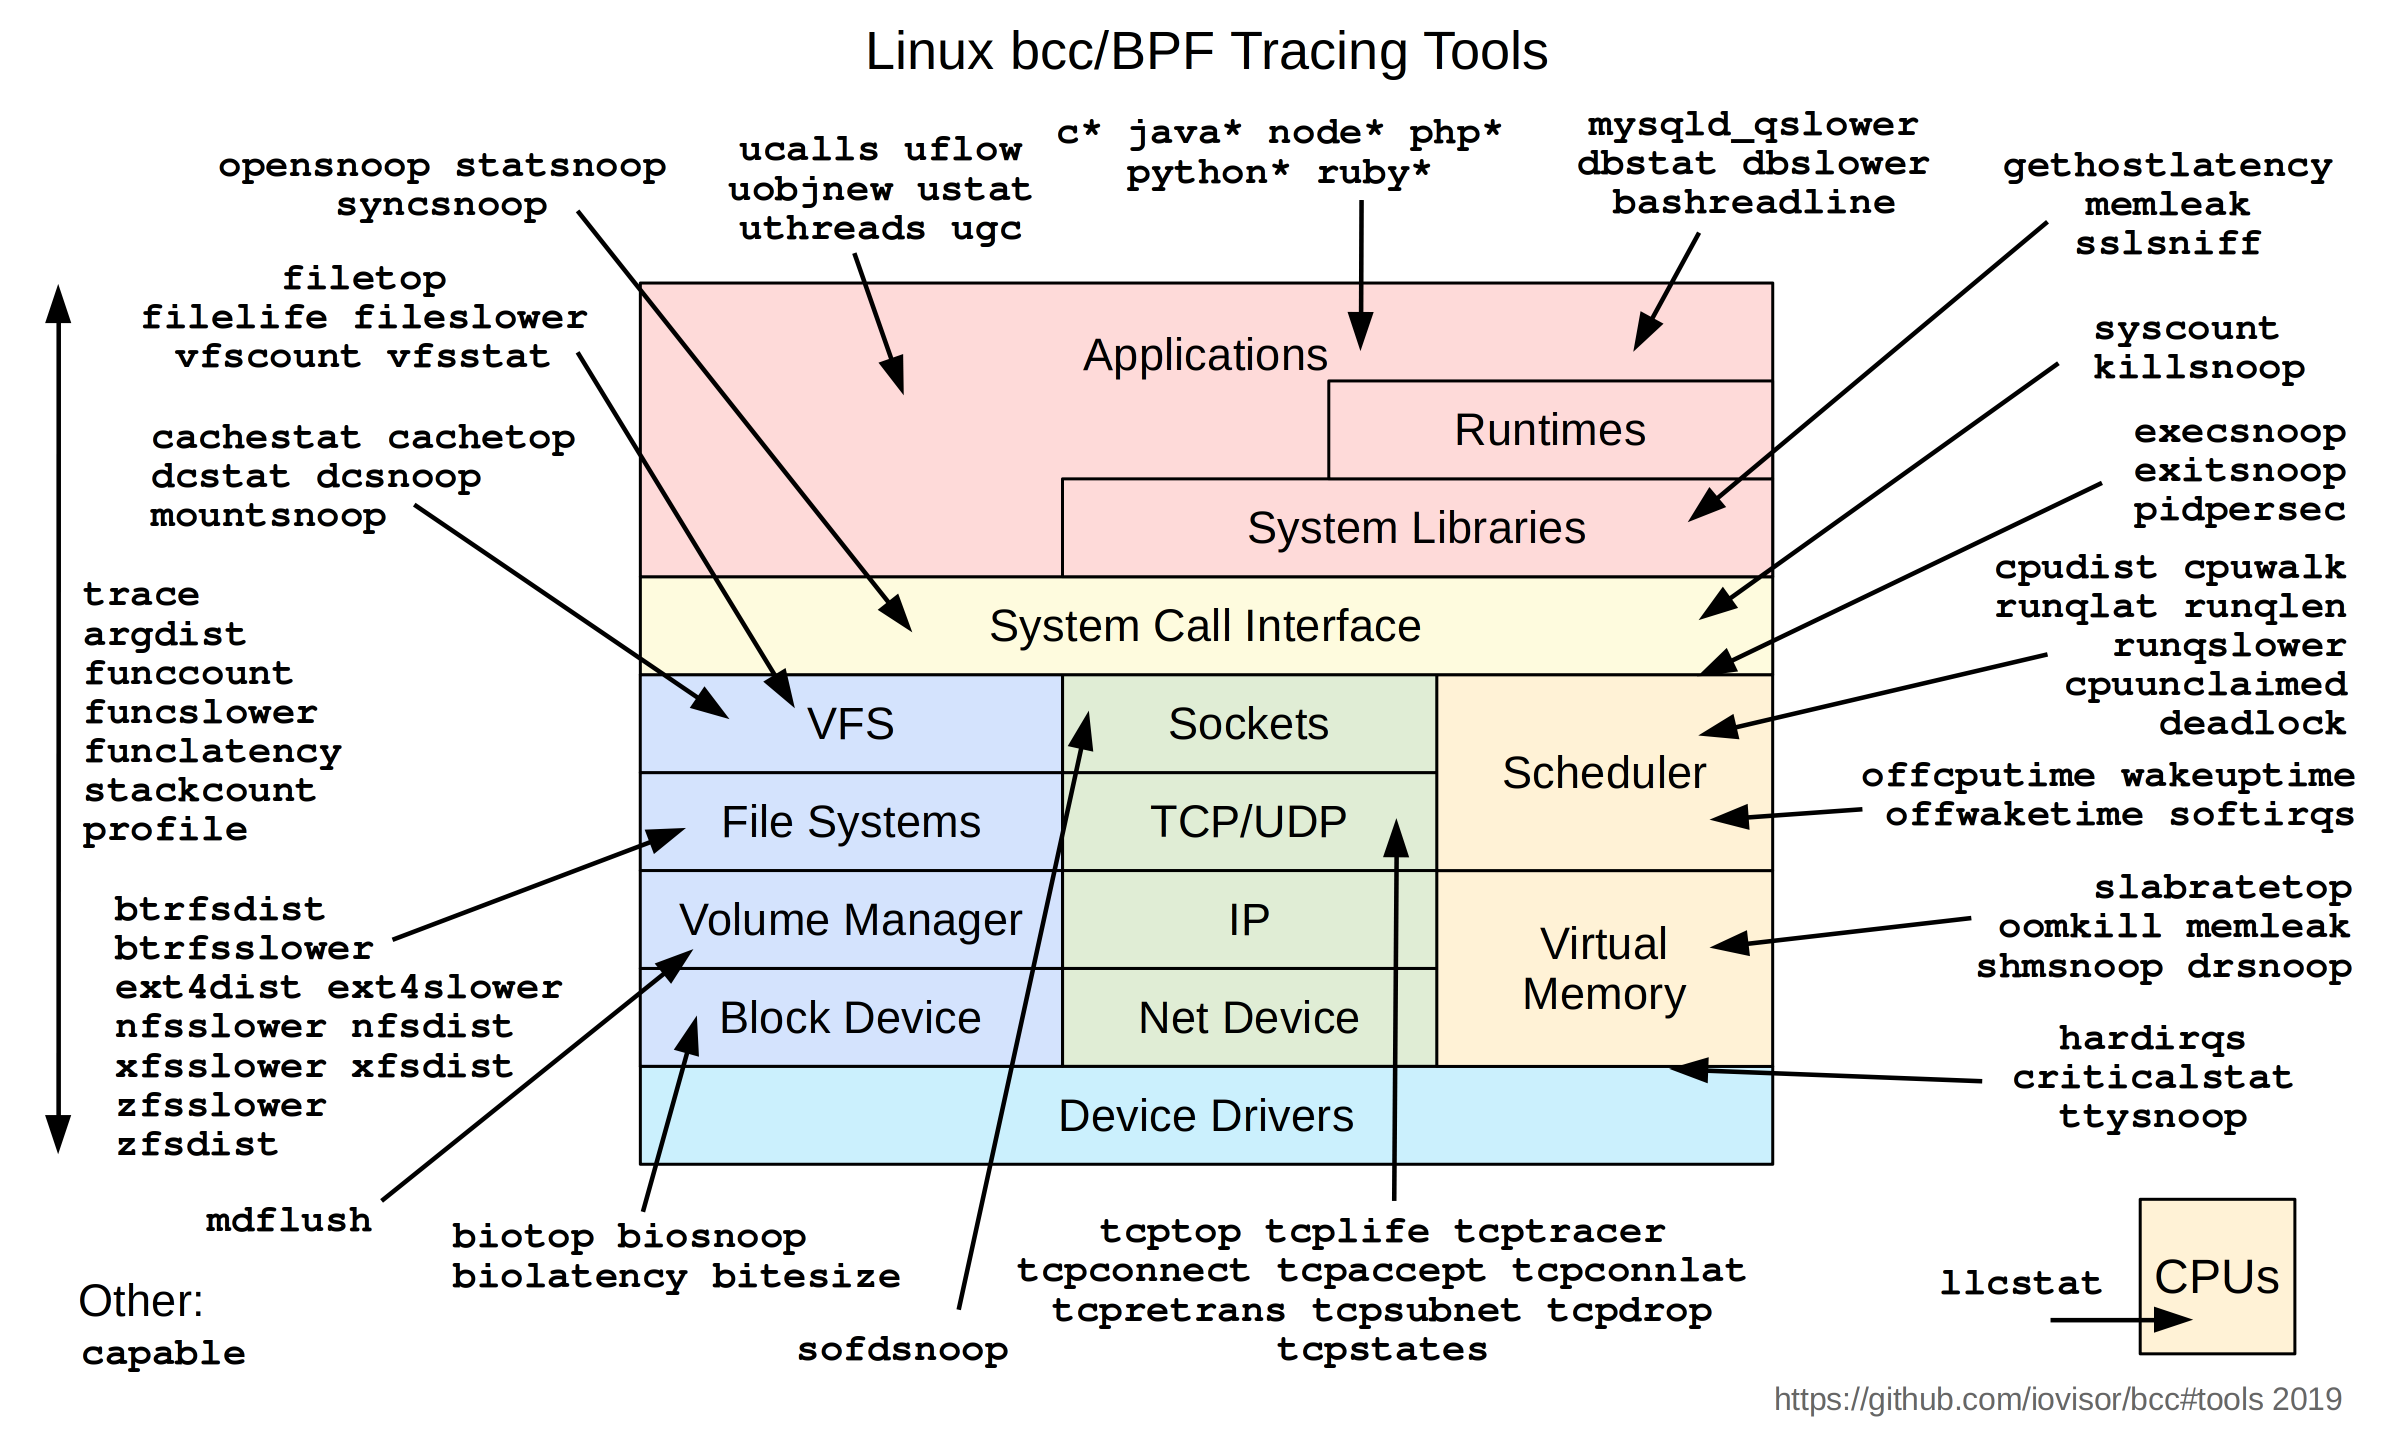
\includegraphics[height=0.8\textheight]{slides/debugging-system-wide-profiling/bcc_tracing_tools_2019.png}\\
    \tiny Image credits: \url{https://www.brendangregg.com/ebpf.html}
  \end{center}
\end{frame}

\begin{frame}[fragile]
  \frametitle{BCC Tools example}
  \begin{itemize}
    \item \code{profile.py} is a CPU profiler allowing to capture stack traces of
          current execution. Its output can be used for flamegraph generation:
  \end{itemize}
  \begin{block}{}
    \begin{minted}[fontsize=\footnotesize]{console}
$ git clone https://github.com/brendangregg/FlameGraph.git
$ profile.py -df -F 99 10 | ./FlameGraph/flamegraph.pl > flamegraph.svg
    \end{minted}
  \end{block}
  \begin{itemize}
    \item \code{tcpconnect.py} script displays all new TCP connections live
  \end{itemize}
  \begin{block}{}
    \begin{minted}[fontsize=\footnotesize]{console}
$ tcpconnect
PID    COMM         IP SADDR            DADDR            DPORT
220321 ssh          6  ::1              ::1              22   
220321 ssh          4  127.0.0.1        127.0.0.1        22   
17676  Chrome_Child 6  2a01:cb15:81e4:8100:37cf:d45b:d87d:d97d 2606:50c0:8003::154 443  
[...]
    \end{minted}
  \end{block}
  \begin{itemize}
    \item And much more to discover at \url{https://github.com/iovisor/bcc}
  \end{itemize}
\end{frame}

\begin{frame}[fragile]
  \frametitle{Using BCC with python}
  \begin{itemize}
    \item BCC exposes a \code{bcc} module, and especially a \code{BPF} class
    \item eBPF programs are written in C and stored either in external files
    or directly in a python string.
    \item When an instance of the \code{BPF} class is created and fed with the
    program (either as string or file), it automatically builds, loads, and
    possibly attaches the program
    \item There are multiple ways to attach a program:
    \begin{itemize}
      \item By using a proper program name prefix, depending on the targeted
      attach point (and so the attach step is performed automatically)
      \item By explicitly calling the relevant attach method on the \code{BPF}
      instance created earlier
    \end{itemize}
  \end{itemize}
\end{frame}

\begin{frame}[fragile]
  \frametitle{Using BCC with python}
  \begin{itemize}
    \item Hook with a {\em kprobe} on the \code{clone()} system call and display \verb+"Hello, World!"+ each
          time it is called
  \end{itemize}
  \begin{block}{}
    \begin{minted}[fontsize=\small]{python}
#!/usr/bin/env python3

from bcc import BPF

# define BPF program
prog = '''
int hello(void *ctx) {
    bpf_trace_printk("Hello, World!\\n");
    return 0;
}
'''
# load BPF program
b = BPF(text=prog)
b.attach_kprobe(event=b.get_syscall_fnname("clone"), fn_name="hello")
    \end{minted}
  \end{block}
\end{frame}

\setuplabframe
{Custom eBPF tool with BCC}
{
	\begin{itemize}
		\item Creating custom tracing tools with BCC framework
	\end{itemize}
}


\begin{frame}[fragile]
  \frametitle{libbpf}
  \begin{itemize}
    \item Instead of using a high level framework like BCC, one can use libbpf to
    build custom tools with finer control over every aspect of the program.
    \item libbpf is a C-based library that aims to ease eBPF programming thanks
    to the following features:
    \begin{itemize}
      \item userspace APIs to handle open/load/attach/teardown of bpf programs
      \item userspace APIs to interact with attached programs
      \item eBPF APIs to ease eBPF program writing
    \end{itemize}
    \item Packaged in many distributions and build systems (e.g.: Buildroot)
    \item Learn more at \url{https://libbpf.readthedocs.io/en/latest/}
  \end{itemize}
\end{frame}

\begin{frame}[fragile]
  \frametitle{eBPF programming with libbpf (1/2)}
  \begin{block}{\code{my_prog.bpf.c}}
    \begin{minted}[fontsize=\tiny]{C}
      #include <linux/bpf.h>
      #include <bpf/bpf_helpers.h>
      #include <bpf/bpf_tracing.h>

      #define TASK_COMM_LEN 16
      struct {
        __uint(type, BPF_MAP_TYPE_ARRAY);
        __type(key, __u32);
        __type(value, __u64);
        __uint(max_entries, 1);
      } counter_map SEC(".maps");

      struct sched_switch_args {
        unsigned long long pad;
        char prev_comm[TASK_COMM_LEN];
        int prev_pid;
        int prev_prio;
        long long prev_state;
        char next_comm[TASK_COMM_LEN];
        int next_pid;
        int next_prio;
      };
    \end{minted}
  \end{block}

  \begin{itemize}
  \item The fields to define in the \code{*_args} structure are obtained
    from the event description in \code{/sys/kernel/tracing/events} (see
    \href{https://elixir.bootlin.com/linux/v6.12/source/tools/testing/selftests/bpf/progs/test_stacktrace_map.c#L41}
         {this example})
  \end{itemize}
\end{frame}

\begin{frame}[fragile]
  \frametitle{eBPF programming with libbpf (2/2)}
  \begin{block}{\code{my_prog.bpf.c}}
    \begin{minted}[fontsize=\tiny]{C}
      SEC("tracepoint/sched/sched_switch")
      int sched_tracer(struct sched_switch_args *ctx)
      {
        __u32 key = 0;
        __u64 *counter;
        char *file;

        char fmt[] = "Old task was %s, new task is %s\n";
        bpf_trace_printk(fmt, sizeof(fmt), ctx->prev_comm, ctx->next_comm);

        counter = bpf_map_lookup_elem(&counter_map, &key);
        if(counter) {
                *counter += 1;
                bpf_map_update_elem(&counter_map, &key, counter, 0);
        }

        return 0;
      }

      char LICENSE[] SEC("license") = "Dual BSD/GPL";
    \end{minted}
  \end{block}
\end{frame}


\begin{frame}[fragile]
  \frametitle{Building eBPF programs}
  \begin{itemize}
    \item An eBPF program written in C can be built into a loadable object
    thanks to clang:
    \begin{block}{}
      \begin{minted}{console}
        $ clang -target bpf -O2 -g -c my_prog.bpf.c -o my_prog.bpf.o
      \end{minted}
    \end{block}
    \begin{itemize}
        \item The \code{-g} option allows to add debug information as well as
        BTF information
    \end{itemize}
    \item GCC can be used too with recent versions
    \begin{itemize}
      \item the toolchain can be installed with the \code{gcc-bpf} package in
      Debian/Ubuntu
      \item it exposes the \code{bpf-unknown-none} target
    \end{itemize}
    \item To easily manipulate this program with a userspace program based on libbpf,
    we need "skeleton" APIs, which can be generated with to \code{bpftool}
  \end{itemize}
\end{frame}

\begin{frame}[fragile]
  \frametitle{bpftool}
  \begin{itemize}
    \item \code{bpftool} is a command line tool allowing to interact with bpf
    object files and the kernel to manipulate bpf programs:
    \begin{itemize}
      \item Load programs into the kernel
      \item List loaded programs
      \item Dump program instructions, either as BPF code or JIT code
      \item List loaded maps
      \item Dump map content
      \item Attach programs to hooks (so they can run)
      \item etc
    \end{itemize}
    \item You may need to mount the bpf filesystem to be able to pin a program
    (needed to keep a program loaded after bpftool has finished running):
    \begin{block}{}
      \begin{minted}{console}
        $ mount -t bpf none /sys/fs/bpf
      \end{minted}
    \end{block}
  \end{itemize}
\end{frame}

\begin{frame}[fragile]
  \frametitle{bpftool}
  \begin{itemize}
    \item List loaded programs
  \end{itemize}
  \begin{block}{}
    \fontsize{10}{10}\selectfont
    \begin{minted}{console}
$ bpftool prog
348: tracepoint  name sched_tracer  tag 3051de4551f07909  gpl
loaded_at 2024-08-06T15:43:11+0200  uid 0
xlated 376B  jited 215B  memlock 4096B  map_ids 146,148
btf_id 545
    \end{minted}
  \end{block}
  \begin{itemize}
    \item Load and attach a program
  \end{itemize}
  \begin{block}{}
    \fontsize{10}{10}\selectfont
    \begin{minted}{console}
$ mkdir /sys/fs/bpf/myprog
$ bpftool prog loadall trace_execve.bpf.o /sys/fs/bpf/myprog autoattach
    \end{minted}
  \end{block}
  \begin{itemize}
    \item Unload a program
  \end{itemize}
  \begin{block}{}
    \fontsize{10}{10}\selectfont
    \begin{minted}{console}
$ rm -rf /sys/fs/bpf/myprog
    \end{minted}
  \end{block}
\end{frame}

\begin{frame}[fragile]
  \frametitle{bpftool}
  \begin{itemize}
    \item Dump a loaded program
  \end{itemize}
  \begin{block}{}
    \fontsize{8}{8}\selectfont
    \begin{minted}{console}
$ bpftool prog dump xlated id 348
int sched_tracer(struct sched_switch_args * ctx):
; int sched_tracer(struct sched_switch_args *ctx)
  0: (bf) r4 = r1
  1: (b7) r1 = 0
; __u32 key = 0;
  2: (63) *(u32 *)(r10 -4) = r1
; char fmt[] = "Old task was %s, new task is %s\n";
  3: (73) *(u8 *)(r10 -8) = r1
  4: (18) r1 = 0xa7325207369206b
  6: (7b) *(u64 *)(r10 -16) = r1
  7: (18) r1 = 0x7361742077656e20
[...]
    \end{minted}
  \end{block}
  \begin{itemize}
    \item Dump eBPF program logs
  \end{itemize}
  \begin{block}{}
    \fontsize{6}{6}\selectfont
    \begin{minted}{console}
$ bpftool prog tracelog
kworker/u80:0-11  [013] d..41  1796.003605: bpf_trace_printk: Old task was kworker/u80:0, new task is swapper/13
<idle>-0          [013] d..41  1796.003609: bpf_trace_printk: Old task was swapper/13, new task is kworker/u80:0
sudo-18640        [010] d..41  1796.003613: bpf_trace_printk: Old task was sudo, new task is swapper/10
<idle>-0          [010] d..41  1796.003617: bpf_trace_printk: Old task was swapper/10, new task is sudo
[...]
    \end{minted}
  \end{block}
\end{frame}

\begin{frame}[fragile]
  \frametitle{bpftool}
  \begin{itemize}
    \item List created maps
  \end{itemize}
  \begin{block}{}
    \fontsize{9}{9}\selectfont
    \begin{minted}{console}
$ bpftool map
80: array  name counter_map  flags 0x0
    key 4B  value 8B  max_entries 1  memlock 256B
    btf_id 421
82: array  name .rodata.str1.1  flags 0x80
    key 4B  value 33B  max_entries 1  memlock 288B
    frozen
96: array  name libbpf_global  flags 0x0
    key 4B  value 32B  max_entries 1  memlock 280B
[...]
    \end{minted}
  \end{block}
  \begin{itemize}
    \item Show a map content
  \end{itemize}
  \begin{block}{}
    \fontsize{9}{9}\selectfont
    \begin{minted}{console}
$ sudo bpftool map dump id 80
[{
  "key": 0,
  "value": 4877514
  }
]
    \end{minted}
  \end{block}
\end{frame}

\begin{frame}[fragile]
  \frametitle{bpftool}
  \begin{itemize}
    \item Generate libbpf APIs to manipulate a program
  \end{itemize}
  \begin{block}{}
    \fontsize{9}{9}\selectfont
    \begin{minted}{console}
$ bpftool gen skeleton trace_sched_switch.bpf.o name trace_sched_switch \
  > trace_sched_switch.skel.h
    \end{minted}
  \end{block}
  \begin{itemize}
    \item We can then write our userspace program and benefit from high level
    APIs to manipulate our eBPF program:
    \begin{itemize}
      \item instantiation of a global context object which will have references
      to all of our programs, maps, links, etc
      \item loading/attaching/unloading of our programs
      \item eBPF program directly embedded in the generated header as a byte
      array
    \end{itemize}
  \end{itemize}
\end{frame}

\begin{frame}[fragile]
  \frametitle{Userspace code with libbpf}
  \begin{block}{}
    \begin{minted}[fontsize=\tiny]{C}
      #include <stdlib.h>
      #include <stdio.h>
      #include <unistd.h>
      #include "trace_sched_switch.skel.h"

      int main(int argc, char *argv[])
      {
          struct trace_sched_switch *skel;
          int key = 0;
          long counter = 0;

          skel = trace_sched_switch__open_and_load();
          if(!skel)
              exit(EXIT_FAILURE);
          if (trace_sched_switch__attach(skel)) {
              trace_sched_switch__destroy(skel);
              exit(EXIT_FAILURE);
          }

          while(true) {
              bpf_map__lookup_elem(skel->maps.counter_map, &key, sizeof(key), &counter, sizeof(counter), 0);
              fprintf(stderr, "Scheduling switch count: %d\n", counter);
              sleep(1);
          }

          return 0;
      }
    \end{minted}
  \end{block}
\end{frame}

\begin{frame}
  \frametitle{eBPF programs portability (1/2)}
  \begin{itemize}
    \item Kernel internals, contrary to userspace APIs, do not expose stable APIs.
    This means that an eBPF program manipulating some kernel data may not work
    with another kernel version
    \item The CO-RE (Compile Once - Run Everywhere) approach aims to solve this issue
    and make programs portable between \textbf{kernel versions}. It relies on
    the following features:
    \begin{itemize}
      \item your kernel must be built with
      \kconfigval{CONFIG_DEBUG_INFO_BTF}{y} to have BTF data embedded. BTF is a
      format similar to dwarf which encodes data layout and function
      signatures in an efficient way.
      \item your eBPF compiler must be able to emit BTF relocations (both clang
      and GCC are capable of this on recent versions, with the \code{-g} argument)
      \item you need a BPF loader capable of processing BPF programs based on BTF data and
      adjust accordingly data access: \code{libbpf} is the de-facto standard bpf
      loader
      \item you then need eBPF APIs to read/write to CO-RE relocatable
      variables. libbpf provides such helpers, like \code{bpf_core_read}
    \end{itemize}
    \item To learn more, take a look at
    \href{https://nakryiko.com/posts/bpf-core-reference-guide/}{Andrii
    Nakryiko's CO-RE guide}
  \end{itemize}
\end{frame}

\begin{frame}
  \frametitle{eBPF programs portability (2/2)}
  \begin{itemize}
    \item Despite CO-RE, you may still face different constraints on different
    kernel versions, because of major features introduction or change, since
    the eBPF subsystem keeps receiving frequent updates:
    \begin{itemize}
      \item eBPF tail calls (which allow a program to call a function) have
      been added in version 4.2, and allow to call another program only since
      version 5.10
      \item eBPF spin locks have been added in version 5.1 to prevent
      concurrent access to maps shared between CPUs.
      \item Different attach types keep being added, but possibly on different
      kernel versions when it depends on the architecture: fentry/fexit attach
      points have been added in kernel 5.5 for x86 but in 6.0 for arm32.
      \item Any kind of loop (even bounded) was forbidden until version 5.3
      \item \code{CAP_BPF} capability, allowing a process to perform eBPF tasks, has
      been added in version 5.8
    \end{itemize}
  \end{itemize}
\end{frame}

\begin{frame}[fragile]
\frametitle{eBPF for tracing/profiling}
  \begin{itemize}
    \item eBPF is a very powerful framework to spy on kernel internals: thanks
    to the wide variety of attach point, you can expose almost any kernel code path and data.
    \item In the meantime, eBPF programs remain isolated from kernel code,
    which makes it safe (compared to kernel development) and easy to use.
    \item Thanks to the in-kernel interpreter and optimizations like JIT compilation, eBPF is very well
    suited for tracing or profiling with low overhead, even in production
    environments, while being very flexible.
    \item This is why eBPF adoption level keeps growing for debugging, tracing
    and profiling in the Linux ecosystem. As a few examples, we find eBPF usage in:
    \begin{itemize}
      \item tracing frameworks like \href{https://github.com/iovisor/bcc}{BCC}
      and \href{https://github.com/bpftrace/bpftrace}{bpftrace}
      \item network infrastructure components, like
      \href{https://github.com/cilium/cilium}{Cilium} or \href{https://github.com/projectcalico/calico}{Calico}
      \item network packet tracers, like
      \href{https://github.com/cilium/pwru}{pwru} or
      \href{https://github.com/feiskyer/dropwatch}{dropwatch}
      \item And many more, check \href{https://ebpf.io/applications/}{ebpf.io}
      for more examples
    \end{itemize}
  \end{itemize}
\end{frame}

\begin{frame}[fragile]
  \frametitle{eBPF: resources}
  \begin{itemize}
     \item libbpf-bootstrap: \url{https://github.com/libbpf/libbpf-bootstrap}
    \item A Beginner’s Guide to eBPF Programming - Liz Rice, 2020
    \begin{itemize}
      \item Video: \url{https://www.youtube.com/watch?v=lrSExTfS-iQ}
      \item Resources: \url{https://github.com/lizrice/ebpf-beginners}
    \end{itemize}
  \end{itemize}
  \begin{center}
     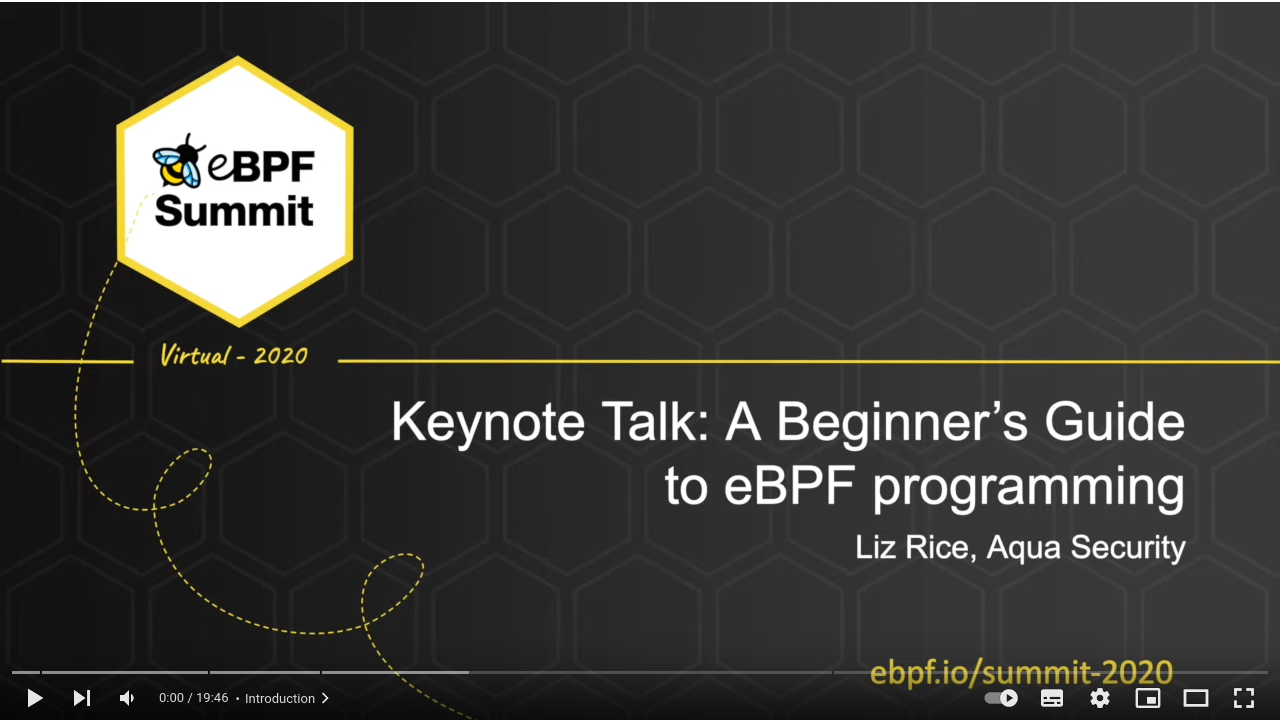
\includegraphics[height=0.4\textheight]{slides/debugging-system-wide-profiling/ebpf_liz_rice_2020.png}
  \end{center}
\end{frame}

\setuplabframe
{Advanced eBPF development}
{
  Porting our custom tracing tool for embedded use case
  \begin{itemize}
    \item Converting a BCC script to libbpf
    \item Bringing advanced features to the tool
  \end{itemize}
}

\subsection{Choosing the right tool}

\begin{frame}[fragile]
  \frametitle{Choosing the right tool}
  \begin{itemize}
    \item Before starting to profile or trace, one should know which type of
          tool to use.
    \item This choice is guided by the level of profiling
    \item Often start by analyzing/optimizing the application level using
          application tracing/profiling tools (valgrind, perf, etc).
    \item Then analyze user space + kernel performance
    \item Finally, trace or profile the whole system if the performance problems
          happens only when running under a loaded system.
    \begin{itemize}
      \item For "constant" load problems, snapshot tools works fine.
      \item For sporadic problems, record traces and analyze them.
    \end{itemize}
  \item If you happen to have a complex setup that you often have to bring up,
  it is likely a sign that you want to ease this setup with some custom tooling:
  scripting, custom traces, eBPF, etc
  \end{itemize}
\end{frame}
